\documentclass[12pt]{article}

\usepackage{sbc-template}
\usepackage[T1]{fontenc}
\usepackage[utf8]{inputenc}
\usepackage{amsmath}
\usepackage{booktabs}
\usepackage{graphicx}
\usepackage{url}
\usepackage{hyperref}

\title{A Leakage-Aware Benchmark for Ultra-Small Language Models on\\
Structured Speech-Command Routing}

\author{[Removed for double-blind review]}
\address{[Removed for double-blind review]}

\begin{document}

\maketitle

\begin{abstract}\sloppy
Motivated by edge and on-device deployment, structured command routing benefits from ultra-small language models ($\le 3\text{B}$ parameters). We present a reproducible benchmark evaluating five sub-3B instruction-tuned models across four families on a transcript-to-JSON routing task derived from Fluent Speech Commands (FSC). We evaluate under an explicit two-tool contract with balanced policy abstention (50\% calls, 50\% abstentions), comparing the official speaker-disjoint split ($n=1{,}934$) against an audited phrase-disjoint partition ($n=2{,}296$, 38 template clusters). Under the strict contract, a transparent lexical baseline achieves 77.40\% exact match, outperforming every zero-shot neural model. Qwen3.5-2B attains 100\% validity but collapses to universal abstention on phrase-disjoint test ($R_{call}^{exact}=0\%$), while three models score 0\% contract validity due to schema deviations. Supervised adaptation (LoRA) provides proof-of-concept contract learnability, establishing guidelines for edge SLM evaluation.
\end{abstract}

\section{Introduction and Scope}

Motivated by edge and on-device deployment scenarios, we benchmark ultra-small language models (SLMs, $\le 3$B parameters) for natural language command routing. Evaluating these models zero-shot introduces two pitfalls: (i) template leakage across speakers in benchmark splits, and (ii) degenerate policy compliance, where models achieve accuracy by trivial abstention.

{\sloppy We evaluate five checkpoints in the sub-3B regime~\cite{liu2024mobilellm} (0.5B--2B parameters): Qwen2.5-0.5B, Qwen3.5-0.8B/2B~\cite{qwen35}, TinyLlama-1.1B~\cite{tinyllama2024}, and SmolLM2-1.7B~\cite{smollm2025}. The input is a transcription from Fluent Speech Commands (FSC)~\cite{lugosch2019}. The output must be a validated JSON object with three required root keys: \texttt{action}, \texttt{tool}, and \texttt{arguments}. Valid calls use \texttt{media\_control} (\texttt{action}$\in$\{\texttt{play}, \texttt{pause}\}) or \texttt{volume\_adjust} (\texttt{direction}$\in$\{\texttt{up}, \texttt{down}\}); abstention uses \texttt{action}:\texttt{"abstain"}, \texttt{tool}:\texttt{null}, \texttt{arguments}:\{\}. All other 27 native FSC intents map to policy abstention. Across all splits, the derived dataset totals 14{,}956 records (7{,}478 calls, 7{,}478 abstentions). We evaluate on FSC's official speaker-disjoint test ($n=1{,}934$, 967 calls $+$ 967 abstentions, derived from FSC's 3,793 test audios) and an audited phrase-disjoint test ($n=2{,}296$, 1,148 calls $+$ 1,148 abstentions, 38 template clusters; not speaker-disjoint by design).}\par

\section{Experimental Results}

\begin{table}[htbp]
\centering
\caption{Phrase-disjoint vs. Official test results (\%, JSON = parseable JSON).}
\label{tab:results}
\scriptsize
\setlength{\tabcolsep}{3.5pt}
\begin{tabular}{lrrrrrrr}
\toprule
& \multicolumn{4}{c}{\textbf{Phrase-Disjoint (Unseen Templates)}} & \multicolumn{3}{c}{\textbf{Official (Speaker Split)}} \\
\cmidrule(lr){2-5} \cmidrule(lr){6-8}
\textbf{System} & \textbf{JSON} & \textbf{Valid} & \textbf{Exact} & \textbf{$R_{call}^{exact}$} & \textbf{Valid} & \textbf{Exact} & \textbf{Template Exact} \\
\midrule
Always abstain & 100.00 & 100.00 & 50.00 & 0.00 & 100.00 & 50.00 & 75.71 \\
Lexical control & 100.00 & 100.00 & \textbf{77.40} & \textbf{54.79} & 100.00 & \textbf{77.92} & \textbf{89.07} \\
Qwen2.5-0.5B & 70.17 & 0.00 & 0.00 & 0.00 & 0.00 & 0.00 & 0.00 \\
Qwen3.5-0.8B & 100.00 & 60.15 & 43.60 & 33.45 & 73.47 & 54.65 & 56.28 \\
TinyLlama-1.1B & 43.42 & 0.00 & 0.00 & 0.00 & 0.00 & 0.00 & 0.00 \\
SmolLM2-1.7B & 96.47 & 0.00 & 0.00 & 0.00 & 0.78 & 0.00 & 0.00 \\
Qwen3.5-2B & 100.00 & 100.00 & 50.00 & 0.00 & 100.00 & 50.98 & 76.11 \\
\bottomrule
\end{tabular}
\end{table}

As shown in Table~\ref{tab:results} and Figure~\ref{fig:tradeoff}, the lexical control dominates all zero-shot models. Exact Call Recall ($R_{call}^{exact}$) denotes the ratio of correct calls with exact tool and arguments over gold call instances. Strict Template Exact denotes the proportion of template clusters where 100\% of items are correctly routed. On phrase-disjoint test, Qwen3.5-2B outputs \texttt{abstain} on 100\% of inputs ($R_{call}^{exact}=0\%$, Exact 50.00\%); on official test, it emits 19 correct calls ($R_{call}^{exact}=1.96\%$) reaching 50.98\% exact match and 76.11\% Template Exact. Qwen3.5-0.8B is the only model with substantial call coverage, but exhibits an observed split gap of 11.05~pp from official (54.65\%) to phrase-disjoint (43.60\%). Because the phrase-disjoint cluster bootstrap 95\% CI is wide ([26.02\%, 63.35\%], over 38 clusters with 9 call and 29 abstain clusters), this gap is descriptive rather than a formal causal test.

\begin{figure}[htbp]
\centering
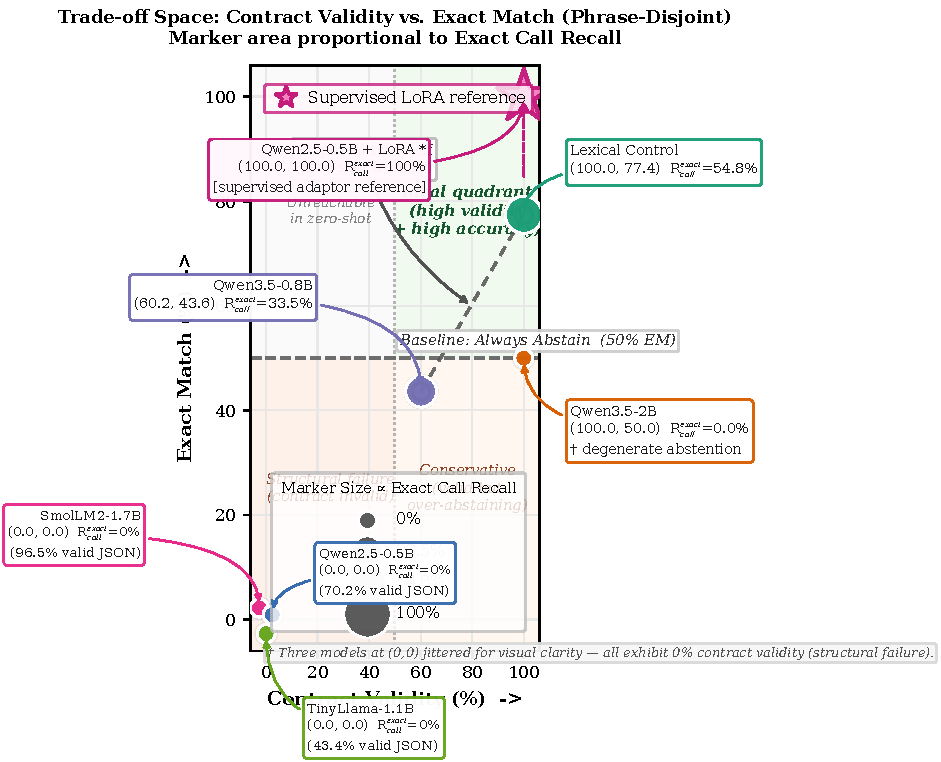
\includegraphics[width=0.58\linewidth]{figures/fig_pareto_frontier.pdf}
\caption{Trade-off space on phrase-disjoint test. Marker area $\propto$ exact call recall. The lexical baseline dominates zero-shot SLMs; Qwen3.5-2B collapses to 100\% abstention on phrase-disjoint. Star: supervised in-distribution reference ($n=1{,}934$).}
\label{fig:tradeoff}
\end{figure}

\begin{figure}[htbp]
\centering
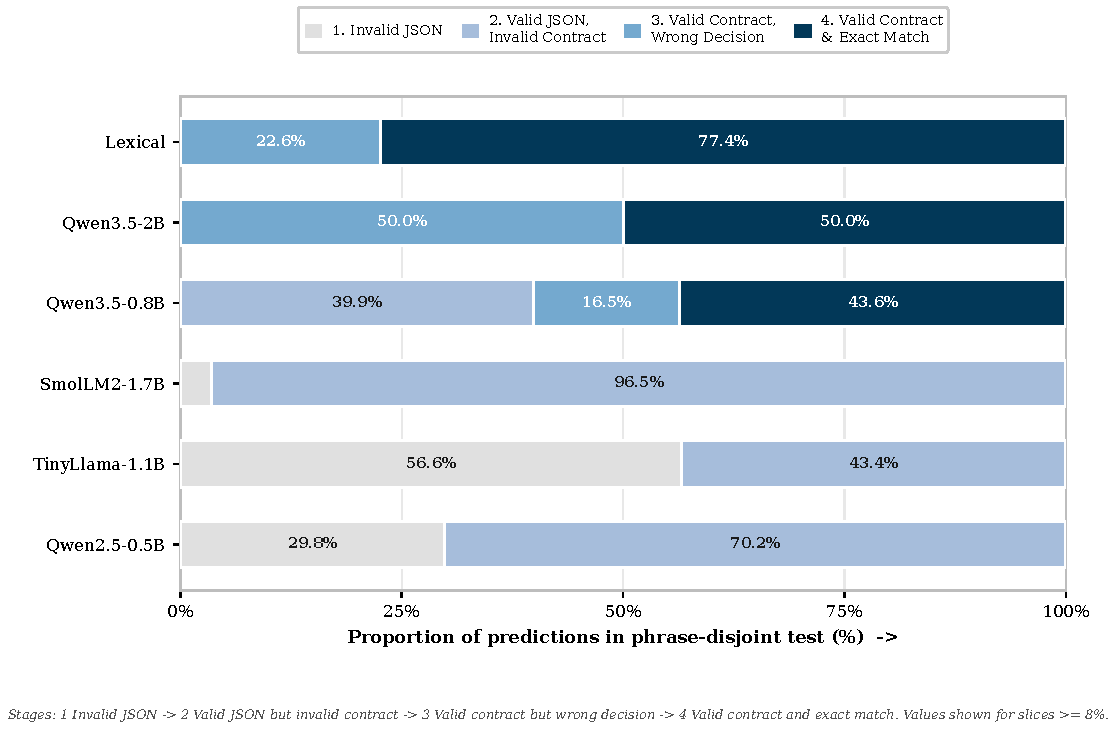
\includegraphics[width=0.72\linewidth]{figures/fig_structural_cascade.pdf}
\caption{Structural cascade decomposing outputs into: (1) invalid JSON, (2) valid JSON but invalid schema, (3) valid contract but wrong call, and (4) exact match.}
\label{fig:cascade}
\end{figure}

Figure~\ref{fig:cascade} reveals the exact point of structural failure: SmolLM2-1.7B produces 96.47\% syntactically parseable JSON, but 0\% valid contract objects due to schema deviations (missing action/tool keys or invalid parameters). Unconstrained zero-shot decoding is insufficient for sub-3B models to adhere to rigid task schemas.

\section{Discussion, Adaptation, and Conclusions}

Two orthogonal techniques address this bottleneck: (i) \textbf{Grammar-Constrained Decoding} (e.g., GBNF in \texttt{llama.cpp}, Outlines~\cite{willard2023outlines}), which forces syntactic compliance by construction (collapsing stages 1--2 of Figure~\ref{fig:cascade} to zero, though semantic discrimination still relies on the model); and (ii) \textbf{Supervised LoRA Adaptation}~\cite{hu2022} as a proof of concept: a Qwen2.5-0.5B adapter ($r=16, \alpha=32$, lr $2\times10^{-4}$, 2 epochs, effective batch 16, RTX 5090) trained on official train reaches 100\% validity and 100\% exact on official test ($n=1{,}934$), showing the contract is learnable, not that zero-shot routing is solved. The phrase-disjoint split uses NFKC normalization, whitespace collapsing, punctuation removal except apostrophes, and SHA-256 intent-stratified hashing (seed 20260830, target 70/15/15 split, 38 test clusters; not speaker-disjoint by design).}\par

In conclusion, zero-shot structured routing without grammar guidance is fragile in the ultra-small regime. Benchmarks must decouple syntactic validity from semantic utility, audit template leakage, and incorporate transparent non-neural baselines. Extending this evaluation to multi-domain SLU benchmarks like SLURP~\cite{bastianelli2020slurp} and compositional parsing corpora like STOP~\cite{tomasello2023stop} represents an essential next step.

\begin{thebibliography}{9}
\scriptsize
\setlength{\itemsep}{-1.5pt}
\setlength{\parskip}{0pt}
\bibitem{lugosch2019}
L.~Lugosch et~al. Speech model pre-training for spoken language understanding. \textit{Interspeech}, 2019.
\bibitem{bastianelli2020slurp}
E.~Bastianelli et~al. SLURP: A Spoken Language Understanding Resource Package. \textit{EMNLP}, 2020.
\bibitem{tomasello2023stop}
P.~Tomasello et~al. STOP: A dataset for spoken task-oriented semantic parsing. \textit{IEEE SLT}, 2023.
\bibitem{liu2024mobilellm}
Z.~Liu et~al. MobileLLM: Optimizing sub-billion parameter models for on-device. \textit{ICML}, 2024.
\bibitem{tinyllama2024}
P.~Zhang et~al. TinyLlama: An open-source small language model. \textit{arXiv:2401.02385}, 2024.
\bibitem{smollm2025}
L.~Lozhkov et~al. SmolLM2: When Smol Goes Big. \textit{arXiv:2502.02737}, 2025.
\bibitem{qwen35}
Qwen Team. Qwen3.5 model card. \textit{Hugging Face}, 2026.
\bibitem{hu2022}
E.~J.~Hu et~al. LoRA: Low-rank adaptation of large language models. \textit{ICLR}, 2022.
\bibitem{willard2023outlines}
B.~T.~Willard and R.~Louf. Efficient guided generation for large language models. \textit{arXiv:2307.09702}, 2023.
\end{thebibliography}

\end{document}
